%% ------------------------------------------------------------------------- %%
\chapter{Fundamentação Teórica}
\label{cap:fundamentacao-teorica}

O problema de remoção de ruído telúrico em sinais astronômicos é de natureza interdisciplinar, o que implica na necessidade de compreender tanto aspectos da teoria astronômica de espectros estelares, quanto aspectos relativos às representações e manipulações computacionais relativas a esse problema.
Neste capítulo são descritos conceitos básicos em espectroscopia astronômica, principalmente estelar, e algoritmos de processamento de sinais digitais utilizados na pesquisa, que em conjunto caracterizam o problema da contaminação telúrica de espectros estelares e sua possível solução através de técnicas de filtragem.

\section{Espectroscopia Astronômica} \label{astronomic-spectroscopy}

% estrelas e radiação eletromagnética
Estrelas são corpos celestes que consistem de esferas de gás ionizado que são mantidos íntegros pela sua gravidade. Uma fonte fundamental de energia das estrelas é através de reações nucleares, principalmente a fusão de hidrogênio em hélio. O produto desta fusão nuclear é emitida para o espaço em parte como radiação eletromagnética \citep{estrelas-ufrgs}.   

% propagação da radiação e chegada na atmosfera/terra
A radiação da estrela se propaga pelo meio interestelar como um fluxo de partículas denominadas fótons. Quando no espaço, estes fótons atingem o limite de velocidade universal, a velocidade da luz $\textit{c} \approx 3 \times 10^8$ m/s. Os fótons se aproximam da Terra nesta velocidade, mas assim que entram em contato com a atmosfera terrestre começam a interagir com moléculas como o oxigênio e o vapor de água \citep{wiki:photon}. Estas moléculas de gás podem absorver os fótons do sinal estelar, e consequentemente, diminuir a quantidade de informação emitida por uma estrela que alcança a superfície terrestre \citep{wiki:telluric-contamination}.

% como a radiação é observada (primeira menção de instrumentos)
Os fótons que alcançam a superfície terrestre são medidos instrumentalmente e constituem uma parte importante da astronomia observacional. Um dos instrumentos utilizados para fazer observações a partir do solo são os espectrógrafos, presentes em muitos telescópios terrestres. 

% como o espectrógrafo gera um espectro e utilização na astronomia (amarra os novos parágrafos com o texto antigo)
Este instrumento tem a capacidade de dividir a radiação eletromagnética de um objeto celeste em seus respectivos comprimentos de onda, resultando em um espectro: um mapa de radiação em função do comprimento de onda. Na astronomia, diversos corpos celestes podem ser o objeto de estudo de observações espectrais, como estrelas, planetas, nebulosas, galáxias e núcleos galácticos ativos.  

% A espectroscopia é a técnica de dividir a luz, ou mais precisamente, a radiação eletromagnética, proveniente de um objeto, em seus comprimentos de onda constituintes, o que resulta na formação de um mapa de radiação em função do comprimento de onda denominado espectro. Quando aplicada na astronomia, a espectroscopia tem como objeto de estudo o espectro de radiação eletromagnética de diversos corpos celestes, como estrelas, planetas, nebulosas, galáxias e núcleos galácticos ativos.

% tipos de espectro
Diferentes tipos de objetos celestes produzem diferentes tipos de espectro:  contínuo, de absorção e de emissão. Um espectro contínuo é uma função que tem como domínio todos os comprimentos de ondas do espectro eletromagnético.
Ele é gerado pela observação de um corpo opaco quente, que seria o equivalente a observar diretamente o núcleo de uma estrela sem intervenção de matéria entre estrela e observador. Um espectro de absorção, ou espectro de linhas escuras, é gerado por um gás transparente frio em frente ao corpo opaco quente e está associado à absorção dos fótons da radiação estelar em determinados comprimentos de onda. E por último, o espectro de emissão, ou espectro de linhas brilhantes, é gerado por um gás transparente que foi excitado por uma fonte de energia próxima, o que resulta na emissão de fótons de comprimentos de onda específicos. A figura \ref{fig:spectrum-types} ilustra os três tipos de espectros. 

\begin{figure}[htb]
\centering
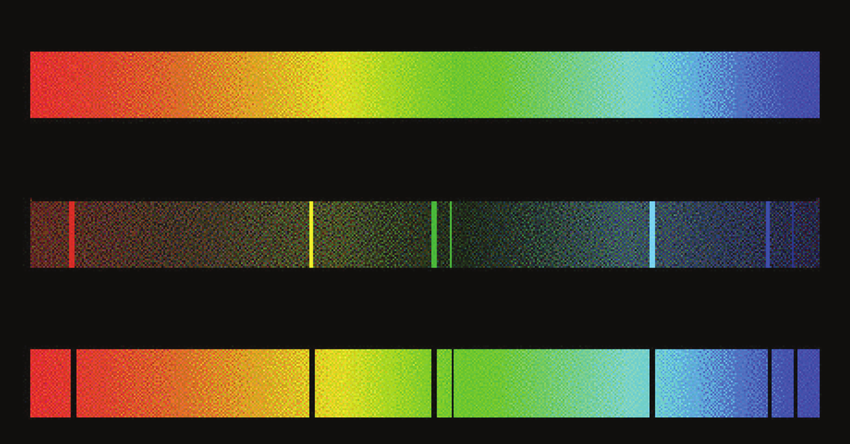
\includegraphics[width=10cm]{figuras/Continuous-spectrum-and-two-types-of-line-spectra.png}
\caption{Os três tipos de espectro: contínuo, de emissão e de absorção \citep{mcgrawhill}}
\label{fig:spectrum-types}
\end{figure}

% espectro estelar
Dentre esta grande variedade de objetos celestes, as estrelas são muito estudadas pelos seus espectros. Por serem objetos quentes, rodeados de gases mais frios, estrelas emitem um espectro de linhas de absorção sobreposto a um espectro contínuo. As linhas de absorção têm comprimentos de onda característicos dos elementos químicos que geraram o espectro. A figura~\ref{fig:vega-spectrum} ilustra o espectro da estrela Vega, cujo formato segue o de um espectro contínuo com a sobreposição de linhas de absorção de hidrogênio, oxigênio e vapor de água.

\begin{figure}[htb]
\centering
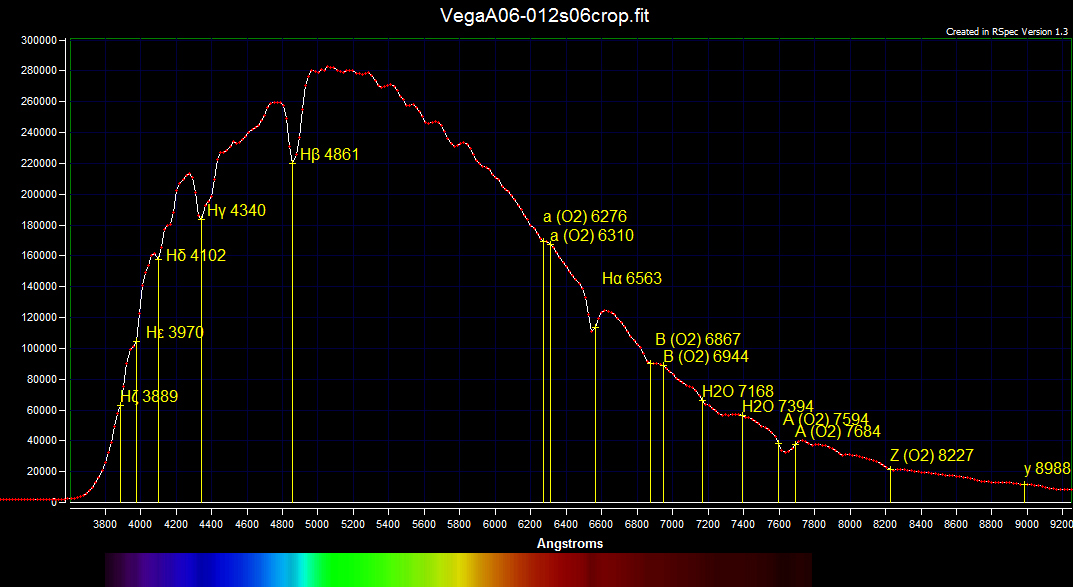
\includegraphics[width=12cm]{figuras/vega_spectrum.jpg}
\caption{O espectro da estrela Vega\citep{vega-spectrum}}
\label{fig:vega-spectrum}
\end{figure}

% história da classificação espectral e estudo dos espectros estelares
No final do século XIX, astrônomos perceberam que a análise cuidadosa do espectro de uma estrela fornece uma riqueza de detalhes sobre ela, incluindo sua temperatura efetiva, velocidade de rotação, velocidade de translação, densidade, composição química e metalicidade. Com a observação rotineira de espectros estelares em grandes números, estes pesquisadores notaram que era possível agrupar as estrelas com base em suas características espectrais, e assim surgiram diversos sistemas de classificação estelar. 

% sistema moderno de classificação espectral estelar
O sistema moderno de classificação de estrelas foi adotado em 1910 e foi criado por um time do observatório da Universidade de Harvard. Este sistema baseia-se nas intensidades relativas das linhas de absorção presentes no espectro. As variações nas linhas espectrais para diferentes estrelas são devidas principalmente à diferença de temperatura das camadas externas de gás na estrela, logo o sistema de classificação espectral é baseado na temperatura efetiva da estrela. 

% classes do sistema de classificação e relação com temperatura
As classes espectrais do sistema, em ordem decrescente de temperatura efetiva da estrela são O, B, A, F, G, K e M, como pode ser visto na tabela~\ref{tab:stellar-temperatures}. Cada uma dessas classes se divide em 10 subclasses (indicadas pelos números de 0 a 9), sendo 0 a mais quente dentro da classe e 9 a mais fria.
Na figura~\ref{fig:stellar-spectrum-types} é possível observar como diferentes linhas de absorção e bandas moleculares variam em intensidade conforme muda a temperatura efetiva, ou tipo espectral, da estrela.

\begin{table}[htb]
\centering
\begin{tabular}{|c|r|}
\hline
\textbf{Tipo Espectral} & \textbf{Temperatura efetiva (K)} \\ \hline
O                       & 30.000                               \\ \hline
B                       & 20.000                               \\ \hline
A                       & 10.000                               \\ \hline
F                       & 7000                                 \\ \hline
G                       & 6000                                 \\ \hline
K                       & 4000                                 \\ \hline
M                       & 3000                                 \\ \hline
\end{tabular}
\caption{A temperatura superficial estelar para cada tipo espectral \citep{iag-stellar-temps}}\label{tab:stellar-temperatures}
\end{table}

\begin{figure}[htb]
\centering
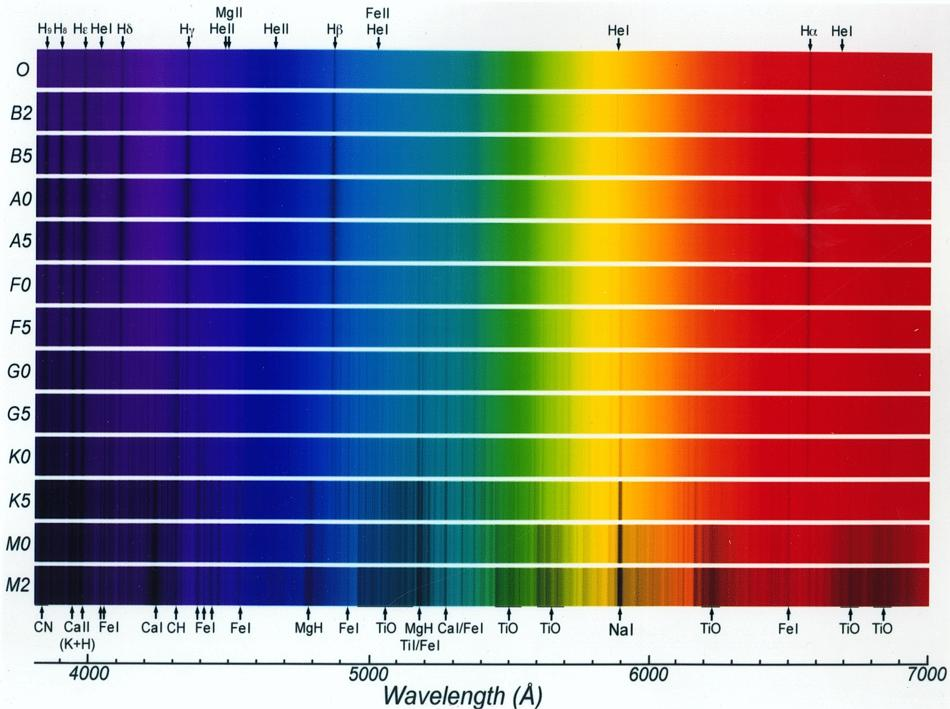
\includegraphics[width=10cm]{figuras/Spectra_Briley.jpg}
\caption{Tipos de espectro estelar \citep{astroprinceton}}
\label{fig:stellar-spectrum-types}
\end{figure}

% finalização da seção: aplicação em pesquisas atuais
% faltando referência
Os tipos espectrais das estrelas continuam sendo uma parte essencial para a pesquisa em astronomia, seja para auxiliar na descoberta de exoplanetas ou na interpretação da história da evolução das galáxias. \pc{senti falta de uma referencia aqui. posso te ajudar, claro.}

\pc{Pergunta para Isa e Marcelo: o quanto voces referenciam artigos em textos da Computacao? No texto abaixo, o meu impulso é adicionar uma referencia para cada conceito, como espectrografo, CCD etc... Posso ajudar nas referencias, claro, mas primeiro gostaria de saber se voces tb estao acostumados a adicionar referencia para quase cada conceito, ou se esse é um viés meu.}

\mqz{Concordamos que qualquer afirmação que não seja clara para nosso leitor em potencial, ou que demande informações adicionais para ser justificada, deveria ser seguida por uma referência. A granularidade de ocorrência dessas referências poderia ser discutida: na passagem a seguir talvez uma referência por parágrafo fosse suficiente, considerando que os parágrafos estejam organizados em torno de uma ideia única central (que pode ser um conceito como sinal espectral ou redução de dados, ou ainda um dispositivo como CCD ou um banco de dados como o XShooter). Minha sensação inicial é que os parágrafos a seguir talvez não estejam tão claramente segmentados, ou seja, amarrados cada um a uma ideia central. Uma técnica que sempre me ajuda é preparar uma lista de ``bullet points'' sobre essas ideias; por exemplo, talvez na sequência a seguir essas ideias-aglutinadoras-de-parágrafos pudessem ser:
\begin{itemize}
    \item espectrógrafo e sinal espectral
    \item redução de dados
    \item descrição da coleção XShooter (isso me pareceria mais natural numa seção sobre datasets, mas talvez pudesse ser introduzida brevemente num parágrafo aqui como elemento auxiliar nas ilustrações dos demais conceitos teóricos).
\end{itemize}
Por sinal, tudo o que aparece nessa seção caberia muito naturalmente (mais naturalmente?) na seção~\ref{astronomic-spectroscopy} ``Espectrografia Astronômica''.}

\section{Redução de Dados}

Estes instrumentos de observação muitas vezes estão munidos de um CCD ou \textit{charge-coupled device}, um sensor eletrônico constituído por vários quadrados fotossensíveis, que registram o sinal em pixels de uma imagem. As imagens resultantes de uma observação do CCD passam por um processo de redução de dados, que envolve a transformação das imagens brutas em dados científicos utilizáveis.   

No caso dos espectros estelares, a redução de dados implica na extração de um espectro unidimensional a partir de uma imagem de CCD da estrela observada, também chamada de estrela de ciência. A figura~\ref{fig:x0319-obs-spectrum} ilustra o espectro de uma estrela da \textit{X-Shooter Spectral Library} \citep{Chen2014TheXS}, uma coleção de estrelas observada pelo espectrógrafo de resolução média \textit{X-Shooter}\footnote{\url{https://www.eso.org/sci/facilities/paranal/instruments/xshooter.html}}, parte do \textit{Very Large Telescope array}\footnote{\url{https://www.eso.org/public/brazil/teles-instr/paranal-observatory/vlt/?lang}} (VLT), localizado no Cerro Paranal, Chile.  

\begin{figure}[htb]
\centering
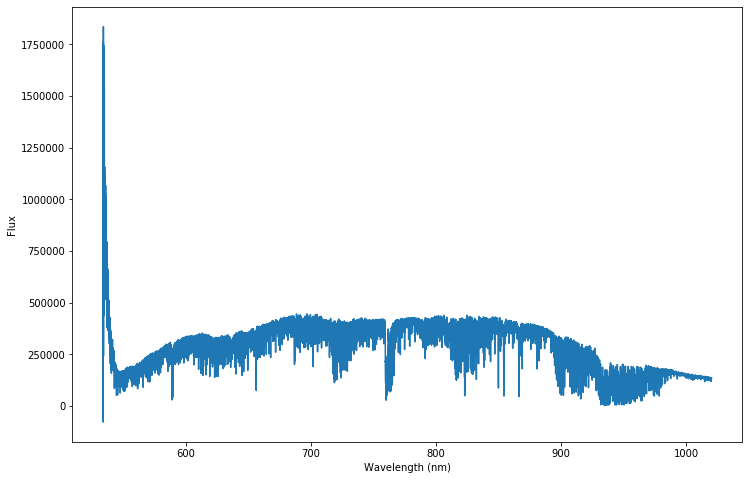
\includegraphics[width=15cm]{figuras/X0319_obs_spectrum.png}
\caption{O espectro observado da estrela X0319}
\label{fig:x0319-obs-spectrum}
\end{figure}

O espectro resultante da redução de dados é unidimensional no domínio do comprimento de onda da estrela e tem sua intensidade representada pelo fluxo. 

O fluxo é capturado em unidades de contagem de fótons, também chamadas de ADUs (\textit{Analog Digital Units}), que são adimensionais. O fluxo de um espectro estelar pode ser reescalonado para o intervalo $[0, 1]$, porém nem sempre isto é feito, como pode ser visto na imagem \ref{fig:x0319-obs-spectrum}. 

Também é possível observar que a figura \ref{fig:x0319-obs-spectrum} tem o formato esperado de um espectro estelar mencionado na seção \ref{astronomic-spectroscopy}: um espectro contínuo com a presença de várias linhas de absorção.


\section{Contaminação Telúrica} \label{telluric-contamination}

Como as estrelas do \textit{X-Shooter Spectral Library}, a maioria das observações astronômicas são feitas em telescópios terrestres, ou seja, a partir do solo. Nesse caso, nem toda luz irradiada por um objeto celestre pode ser capturada pelo espectrógrafo. Isto acontece porque, ao atravessar a atmosfera terrestre, o sinal astronômico interage com moléculas como vapor de água e oxigênio, o que resulta na formação de novas linhas no espectro observado, chamadas de linhas telúricas. 
\pc{acho que cabe mencionar que regioes diferentes de comprimento de onda sao mais ou menos sensiveis aa atmosfera, e mostrar um grafico ilustrando um espectro telurico. pode ser da literatura, assim mostramos um observado (ao contrario dos que voce tem sao modelos). }

As linhas telúricas, quando misturadas no espectro original, contribuem para a criação de uma observação distorcida ou contaminada. A menos que seja corrigida, esta contaminação pode produzir erros de interpretação e ruídos que reduzem a precisão dos dados observados, e consequentemente, dificultam o avanço de diversas pesquisas astronômicas.

Existem alguns procedimentos típicos usados hoje em dia para remover as linhas telúricas de um espectro de ciência. Um método popular consiste em aplicar uma divisão simples entre o espectro da observação e uma referência telúrica, quando satisfeita a condição de que o referencial telúrico tenha as mesmas assinaturas instrumentais do espectro de ciência. \pc{essa ultima frase que eu adicionei tem a ver com alguma conversa que tivemos, o Marcelo explicou disso na lousa. vou rever as conversas e as fotos da lousa pra podermos expandir se / quando necessario}. Esta referência telúrica pode ser obtida de duas maneiras: através da observação de uma estrela padrão, ou pela simulação de um espectro atmosférico teórico, conforme detalhado a seguir.

As estrelas padrão são estrelas quentes em rotação rápida de tipo espectral B ou A. Elas são escolhidas pois seus espectros não possuem características marcantes além de fortes linhas de hidrogênio. Para que o espectro de uma estrela padrão seja usado como uma referência telúrica, é necessário observá-la em condições muito próximas (tempo, posição no céu e condições atmosféricas) daquelas referentes ao espectro de ciência. Contudo, existem várias limitações fundamentais no nível de correção que pode ser obtido com o método da estrela padrão. Primeiramente, características estelares ainda podem estar presentes no espectro da estrela padrão, evidenciando que ela não é um modelo preciso da transmissão radiativa da atmosfera. Além disso, o tempo e a direção de observação das duas estrelas nunca será exatamente o mesmo, o que significa que a assinatura atmosférica de ambos os espectros também será necessariamente diferente.

Devido às limitações das estrelas padrão, foi criado um método mais sofisticado e automatizado para produzir uma referência telúrica: softwares de simulação do espectro atmosférico. Estes softwares utilizam modelos de transmissão radiativa da atmosfera para criar um espectro telúrico sintético, cujas condições de simulação são muito próximas às condições de observação da estrela de ciência. O modelo de transmissão atmosférica mais utilizado hoje em dia é o \textit{Line-By-Line Radiative Transfer Model (LBLRTM)} \citep{2005JQSRT..91..233C}, que fornece cálculos de radiância espectral com precisão e eficiência. Este modelo utiliza o HITRAN \citep{rothman2009hitran}, um acrônimo para \textit{High-resolution Transmission molecular absorption database}, uma base de dados de linhas e parâmetros espectroscópicos. 

Um exemplo de software de simulação do espectro atmosférico é o Molecfit \citep{smette2015molecfit}, uma ferramenta para a modelagem de linhas telúricas desenvolvido por astrônomos do \textit{European Southern Observatory}. De acordo com seus criadores, o Molecfit recupera o perfil atmosférico mais compatível com o instante da observação da estrela de ciência. Isto envolve a utilização de um modelo de transmissão radiativa da atmosfera com uma base de dados espectral para recuperar atributos como a variação na temperatura, pressão e umidade em função da altitude da observação.

Independentemente de como é gerado o referencial telúrico, 
a divisão simples do espectro observado por este referencial indica que a ação da atmosfera na estrela é de natureza linear e multiplicativa. \pc{é mesmo a divisao dos espectros que indica isso? }\mqzinline{Não... conversamos.} Em termos matemáticos, consideramos os espectros de ciência, telúrico e estelar sem contaminação como vetores $o$ (observado), $a$ (atmosfera) e $s$ (estrela), tais que:

\begin{equation*}
    o := \{o_1, o_2, \cdots, o_{n}\} \qquad a := \{a_1, a_2, \cdots, a_{n}\} \qquad s := \{s_1, s_2, \cdots, s_{n}\} 
\end{equation*}

\noindent onde $n$ representa o comprimento igual dos vetores e estes representam valores discretos do fluxo estelar ou atmosférico em intervalos igualmente espaçados de comprimento de onda. A contaminação telúrica do espectro de ciência nesta representação é a multiplicação dos elementos do vetor telúrico pelo estelar:

\begin{equation*}
    o = a \circ s
\end{equation*}

\noindent onde $\circ$ representa o produto de Hadamard, ou o produto par a par dos elementos do vetor. Esta representação tem como objetivo relaxar as restrições físicas do problema, de forma que seja possível aplicar algoritmos nos sinais que dependem da suposição de linearidade da contaminação telúrica.


\section{Similaridade e alinhamento de sinais}

O estudo de séries temporais tem como objetivo extrair estatísticas e características significativas dos dados analisados. Um dos objetivos compreendidos pela análise de séries temporais é a mensuração da similaridade entre duas sequências. Esta medida de similaridade possui diversas aplicações em áreas como reconhecimento de fala, para saber se uma frase corresponde à outra, economia, para analisar similaridades em dados de investimentos de períodos diferentes, e etc. No caso dos espectros estelares, a similaridade entre sinais pode ser útil para alinhar regiões de contaminação atmosférica de moléculas específicas em um espectro de ciência com as regiões a contaminação correspondente no espectro telúrico.

Para se calcular a similaridade entre duas séries temporais pode ser usada a distância euclideana em pares de pontos de cada série que correspondem ao mesmo instante. Esta métrica funcionaria em sinais perfeitamente sincronizados no domínio do tempo e que se movem na mesma velocidade. No caso das sequências estarem dessincronizadas, pontos similares em cada uma delas começam a se afastar uns dos outros e a conclusão equivocada nesse caso é de que os sinais são pouco similares devido ao aumento da distância euclideana.

Um algoritmo mais roubusto utilizado para determinar a similaridade entre duas séries temporais é o \textit{Dynamic Time Warping (DTW)}. Este algoritmo acha uma correspondência ótima entre duas séries temporais, ou quaisquer dados que podem ser representados como sequências lineares, mesmo que estejam dessincronizados. Isto é feito com o deslocamento elástico das sequências para medir a similaridade de trechos com diferentes fases \citep{shou2005fast}. A figura \ref{fig:euclidean-vs-dtw-matching} ilustra como o DTW encontra uma correspondência mais intuitiva do que a correspondência euclideana, juntando regiões das duas sequências com formatos similares mesmo que não estejam perfeitamente alinhadas.

\begin{figure}[htb]
\centering
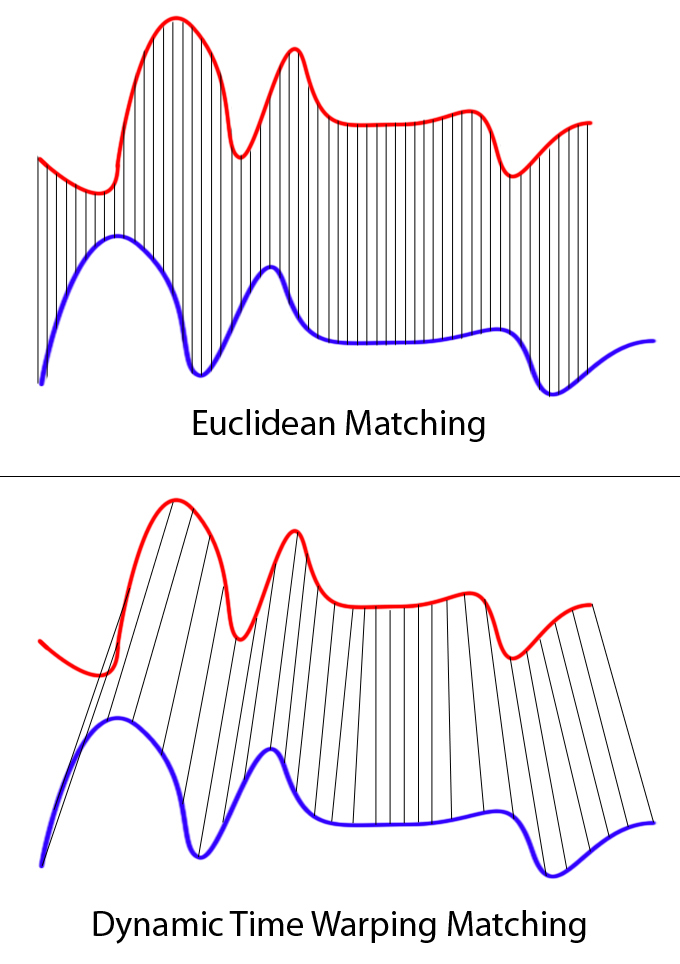
\includegraphics[width=7cm]{figuras/Euclidean_vs_DTW.jpg}
\caption{Diferença entre a correspondência euclideana e da DTW em sinais similares \citep{dtwmatching}}
\label{fig:euclidean-vs-dtw-matching}
\end{figure}

A formulação do problema \citep{salvador2007toward} do \textit{Dynamic Time Warping} é a seguinte: dadas duas sequências $X$ e $Y$, de comprimentos respectivos $n$ e $m$ tal que 

\begin{align*}
    X = \{x_1, x_2, \cdots, x_n\} \\
    Y = \{y_1, y_2, \cdots, y_m\}
\end{align*}

construa um caminho $W$ de comprimento $k$ tal que

\begin{equation*}
    W = \{w_1, w_2, \cdots, w_k\}, \qquad max(n, m) \leq k < n + m
\end{equation*}

e o $k$-ésimo elemento do caminho $W$ é $w_k = (i, j)$ e $i$, $j$ são índices das sequências $X$ e $Y$, respectivamente. O caminho $W$ deve começar em $w_1 = (1, 1)$ e deve terminar em $w_k = (n. m)$, de forma a assegurar que todos os índices das duas sequências serão usados. Também há uma restrição no caminho $W$ que força $i$ e $j$ a serem monótonos não-decrescentes. Em termos matemáticos isso corresponde a

\begin{equation*}
    w_k = (i, j),\, w_{k + 1} = (i', j') \qquad i \leq i' \leq i + 1,\, j\leq j' \leq j + 1
\end{equation*}

Esta descrição do problema possibilita a geração de infinitos caminhos, logo, o objetivo é encontrar o caminho ótimo entre as sequências $X$ e $Y$. O caminho ótimo do algoritmo é o caminho de distância mínima

\begin{equation*}
    dist(W) = \sum_{d=1}^{d=k} dist(w_{di}, w_{dj})
\end{equation*}

onde $dist(W)$ é a distância do caminho $W$ selecionada (tipicamente a euclideana) e $dist(w_{di}, w_{dj})$ é a distância entre um par de dados das sequências $X$ e $Y$ no $d$-ésimo elemento do caminho $W$.

A implementação do algoritmo utiliza o paradigma da programação dinâmica, onde cada instância do problema é resolvida usando soluções de subinstâncias do problema original. O diferencial desta abordagem é que os resultados dos subproblemas são armazenados em uma tabela ou matriz. No caso da DTW é criada uma matrz de distância $D$ de dimensão $n \times m$, onde $D(i, j)$ armazena o valor da distância do caminho mínimo que pode ser construído entre as sequências $X' = \{x_1, \cdots, x_i\}$ e $Y' = \{y_1, \cdots, y_j\}$. Logo, o valor armazenado em $D(n, m)$ representa a distância do caminho mínimo que compreende as duas sequências inteiras. O preenchimento da matriz $D$ é feito com a seguinte lógica

\begin{equation*}
    D(i, j) = dist(i, j) + min\{D(i - 1, j), D(i, j - 1), D(i - 1, j - 1)\}
\end{equation*}

Esta abordagem funciona pois todos os caminhos de sequências que são ligeiramente menores do que as sequências de tamanhos $i$ e $j$ já são conhecidos, logo, a distância armazenada em $D(i, j)$ corresponde à distância mínima entre todos os caminhos possíveis para sequências com um ponto de diferença de $i$ e $j$ mais a distância entre dois pontos $x_i$ e $y_j$. Para que a construção da matriz funcione, o preenchimento deve ser feito uma columna por vez, de baixo para cima e da esquerda para a direita. 

Depois que a matriz $D$ está completa, é necessário encontrar um caminho ótimo entre $D(1, 1)$ e $D(n, m)$. Saindo de $D(n, m)$ é feito um \textit{backtrack} onde em cada elemento da matriz é realizada uma busca gulosa que avalia elementos à esquerda, abaixo e na diagonal inferior esquerda. Dentre estes três avaliados, o elemento com o menor valor é adicionado ao começo do caminho ótimo até o dado momento. Este procedimento é repetido até que o caminho chegue na célula $D(1, 1)$.

\begin{figure}[htb]
\centering
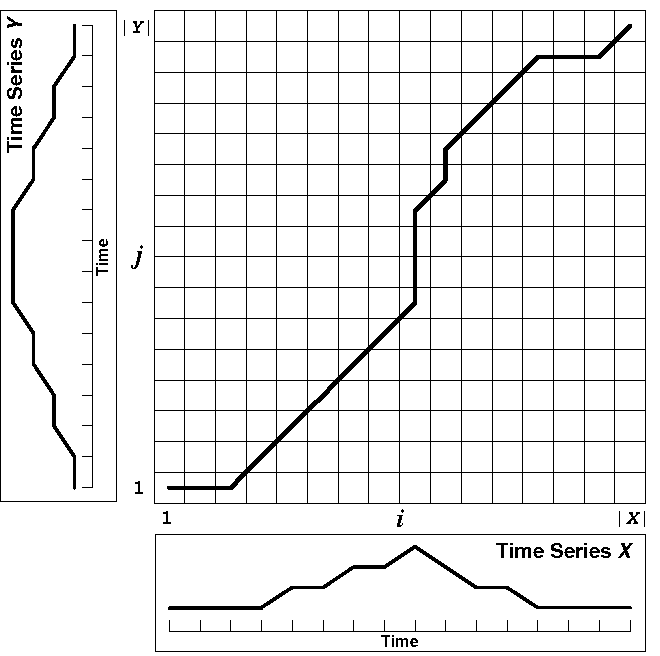
\includegraphics[width=9cm]{figuras/dtw_warp_path.png}
\caption{Uma matriz de similaridade com o caminho ótimo da DTW entre as séries X e Y\citep{salvador2007toward}}
\label{fig:dtw-matrix-and-path}
\end{figure}

O pseudo-código dos procedimentos de preenchimento da matriz \citep{hierarchical-time-clustering} e de \textit{backtracking} que compõem a DTW são dados pelos algoritmos \ref{dtw-matrix} e \ref{dtw-path}.



\begin{algorithm}
\caption{DTW matrix filling}\label{dtw-matrix}
\begin{algorithmic}[1]
\Procedure{DTW}{$x,y$}
    \Comment{Seja $M$ uma matriz bidimensional $n \times m$}
    \State $M[0, 0]\gets 0$
    \For{$i \gets 1$ to $m$}
        \State $M[0, i] \gets \infty$
    \EndFor
    \For{$i \gets 1$ to $n$}
        \State $M[i, 0] \gets \infty$
    \EndFor
    \For{$i \gets 1$ to $n$}
        \For{$j \gets 1$ to $m$}
            \State $d = dist(x[i], y[j])$
            \State $M[i, j] = d + min(M[i-1, j], M[i, j-1], M[i-1, j-1])$
        \EndFor
    \EndFor
\State \textbf{return} $M[n, m]$\Comment{Distância do caminho ótimo}
\EndProcedure
\end{algorithmic}
\end{algorithm}

\begin{algorithm}
\caption{DTW path backtracking}\label{dtw-path}
\begin{algorithmic}[1]
\Procedure{DTW\_path}{$M$}
    \Comment{Seja $P$ uma lista de tuplas}
    \State $i\gets n$
    \State $j\gets m$
    \While{$i \neq 0$ and $j \neq 0$}
        \State P.add(i, j)
        \If{$M[i-1, j-1] \leq M[i-1, j]$ and $M[i-1, j-1] \leq M[i, j-1]$}
            \State $i \gets i - 1$
            \State $j \gets j - 1$
        \ElsIf{$M[i-1, j] \leq M[i-1, j-1]$ and $M[i-1, j] \leq M[i, j-1]$}
            \State $i \gets i - 1$
        \Else
            \State $j \gets j - 1$
        \EndIf
    \EndWhile
\State \textbf{return} $P$\Comment{Índices do caminho ótimo}
\EndProcedure
\end{algorithmic}
\end{algorithm}

É possível analisar a complexidade de tempo e espaço da DTW com o algoritmo de preenchimento da matriz de similaridade. Cada elemento da matriz $n \times m$ é escrito exatamente uma vez em tempo constante, e a matriz inteira é armazenada na memória. Logo, ambas as complexidades são $\mathcal{O}(n * m)$, que no caso de $n = m$, equivale a uma complexidade assintótica $\mathcal{O}(n^2)$. A complexidade de espaço é especialmente proibitiva, visto que sequências com apenas 177 mil elementos geram uma matriz de similaridades que exige \textit{terabytes} de memória para ser armazenada.

A complexidade quadrática tanto em tempo quanto em espaço da DTW, cria a demanda de métodos que consigam acelerar este procedimento. No artigo de \citet{salvador2007toward}, é proposta uma abordagem multinível inspirada no problema da partição de grafos. Essa técnica tende a funcionar bem para problemas muito grandes e de difícil solução por completo. Neste caso, soluções de problemas menores ou parciais podem ser refinadas e combinadas para que se encontre uma boa aproximação da solução do problema original.

O algoritmo proposto, chamado de \textit{FastDTW}, depende de algumas operações-chave: a redução das séries temporais, a projeção do caminho da DTW para maiores resoluções e o refinamento do caminho encontrado. A redução das séries temporais é feita tirando a média de pontos adjacentes e o resultado são vetores com a metade do seu comprimento original. Repete-se esta operação várias vezes para se criar todas as resoluções das séries temporais que serão usadas. O algoritmo quadrático padrão da DTW é utilizado para as séries temporais com menor resolução e o caminho ótimo encontrado é então projetado para a próxima maior resolução que foi computada. Na projeção aplica-se de uma versão restrita da DTW apenas na vizinhança próxima do caminho resultante da projeção, o que não garante que o caminho ótimo será encontrado. Para aumentar as chances de encontrar a solução ótima existe um parâmetro de raio $r$, que representa o número de células adjacentes ao caminho projetado que farão parte da DTW restrita. Este procedimento é repetido para todas as resoluções até finalizar na matriz de resolução original.

O algoritmo usa uma estratégia recursiva, na qual o caso base é o uso da DTW quadrática padrão. Uma análise da complexidade de tempo e espaço do pior caso em que ambas as séries temporais possuem $n$ elementos, resulta em $n(8r + 14)$ para tempo e $n(4r + 7)$ para espaço, ou seja, se o parâmetro $r$ é um valor constante pequeno ($<n$), podemos afirmar que a complexidade assintótica de ambos é $\mathcal{O}(n)$.

Como pode ser visto nos algoritmos \ref{dtw-matrix} e \ref{dtw-path}, as saídas do \textit{Dynamic Time Warping} são a distância e o caminho ótimo entre duas sequências. Neste trabalho foi produzido um algoritmo que tem como objetivo produzir sequências alinhadas. Para isso é utilizado o caminho resultante da DTW e é feita uma aproximação do realinhamento de uma das sequências em relação à outra. O algoritmo implementado, usa os índices repetidos no caminho da DTW e tira a média entre os elementos correspondentes para criar um valor representativo da correspondência de uma região maior de uma sequência com uma região menor de outra.

Em termos matemáticos temos as sequências $a$ e $o$, definidas na seção \ref{telluric-contamination}, queremos $\overline{a}$ que representa a sequência $a$ realinhada em relação à sequência $o$. Para obter este $\overline{a}$, o procedimento é

\begin{equation*}
    \overline{a}_l = \parbox[t]{1.8cm}{média de} \{a_k\}_{k \in L}, \quad  l = 0, \cdots, n
\end{equation*}

\noindent onde

\begin{equation*}
  L = \{m | (m, l) \in P\}
\end{equation*}

\noindent e $P$ representa o caminho resultante da DTW entre $a$ e $o$.

O pseudo-código resultante desta lógica pode ser visto no algoritmo \ref{dtw-realignment}

\begin{algorithm}
\caption{Sequence alignment}\label{dtw-realignment}
\begin{algorithmic}[1]
\Procedure{align\_sequence\_dtw\_path}{$P$, $s$}
    \Comment{Seja $P$ uma lista de tuplas e $s$ o vetor a ser realinhado}
    \State $d \gets \emptyset$ \Comment{Seja $d$ uma associação chave-valor vazia}
    \State $aligned \gets \emptyset$
    \For{$(i, j)$ in $P$}
        \State insere $i$ na lista $d[j]$
    \EndFor
    \For{$(j, lista)$}
        \State $m \gets$ média dos valores de $s$ associados aos índices na lista $d[j]$
        \State $aligned[j] \gets m$
    \EndFor
\State \textbf{return} $aligned$\Comment{Sequência realinhada}
\EndProcedure
\end{algorithmic}
\end{algorithm}
